\PassOptionsToPackage{dvipsnames}{xcolor}
\documentclass[10pt, xcolor={usenames, dvipsnames}]{beamer}

\usepackage[scale=2]{ccicons}
\usepackage{graphicx}
\usepackage{booktabs}
\usepackage{gensymb}
\usepackage{multimedia}
\usepackage{hyperref}
\usepackage{txfonts}
\usepackage{caption}
\usepackage{subcaption}
\usepackage{siunitx}
\usepackage{colortbl}
\usepackage{arydshln}

\usepackage[style=authoryear,backend=biber]{biblatex}
\renewcommand*{\nameyeardelim}{\addcomma\addspace}
\addbibresource{bib/abstract.bib}

% Beamer configuration
\usetheme[sectionpage=progressbar, numbering=counter, progressbar=frametitle]{metropolis}

\usepackage{xfp}
\usepackage{pgfplots}
\usepackage{pgfplotsthemetol}
\usepackage{tikz}
\usetikzlibrary{automata,positioning,arrows,decorations.pathmorphing,calc,patterns,decorations.markings,decorations.shapes,shapes.geometric,matrix}
\usepgfplotslibrary{groupplots,units}
\pgfplotsset{width=7cm,compat=1.18}

\tikzset{paint/.style={ draw=#1, fill=#1 },
         decorate with/.style=
{decorate,decoration={shape backgrounds,shape=#1,shape size=1mm,shape sep=.5cm}}}

% Progressbar
\setbeamercolor{progress bar}{
    fg=TolLightGreen,
    bg=TolLightGreen!50!black!30
}
\makeatletter
    \setlength{\metropolis@titleseparator@linewidth}{2pt}
    \setlength{\metropolis@progressonsectionpage@linewidth}{2pt}
    \setlength{\metropolis@progressinheadfoot@linewidth}{2pt}
\makeatother

% Footer
\setbeamertemplate{frame footer}{Quentin Brateau, ENSTA Bretagne}

% Block fill
\metroset{block=fill}

% Section pages numbering
\makeatletter
\renewcommand{\metropolis@enablesectionpage}{
  \AtBeginSection{
    \ifbeamer@inframe
      \sectionpage
    \else
      \frame[c,plain]{\sectionpage}
    \fi
  }
}
\metropolis@enablesectionpage
\makeatother

% Title
\title{Torpedo-like AUV control}
\date{\today}
\author{Quentin Brateau}
\institute{ENSTA Bretagne}

\titlegraphic{
    \centering
    \begin{tabular}{lllll}
        \href{https://www.defense.gouv.fr/aid}{
\includegraphics[height=0.6cm]{imgs/logo_aid}} &
        \href{https://www.gdr-robotique.org/}{
\includegraphics[height=0.6cm]{imgs/logo_gdr}} &
        \href{https://www.ensta-bretagne.fr/fr/}{
\includegraphics[height=0.6cm]{imgs/logo_ensta}} &
        \href{https://labsticc.fr/fr}{
\includegraphics[height=0.6cm]{imgs/logo_labsticc}} &
        \href{https://www.ensta-bretagne.fr/robex/}{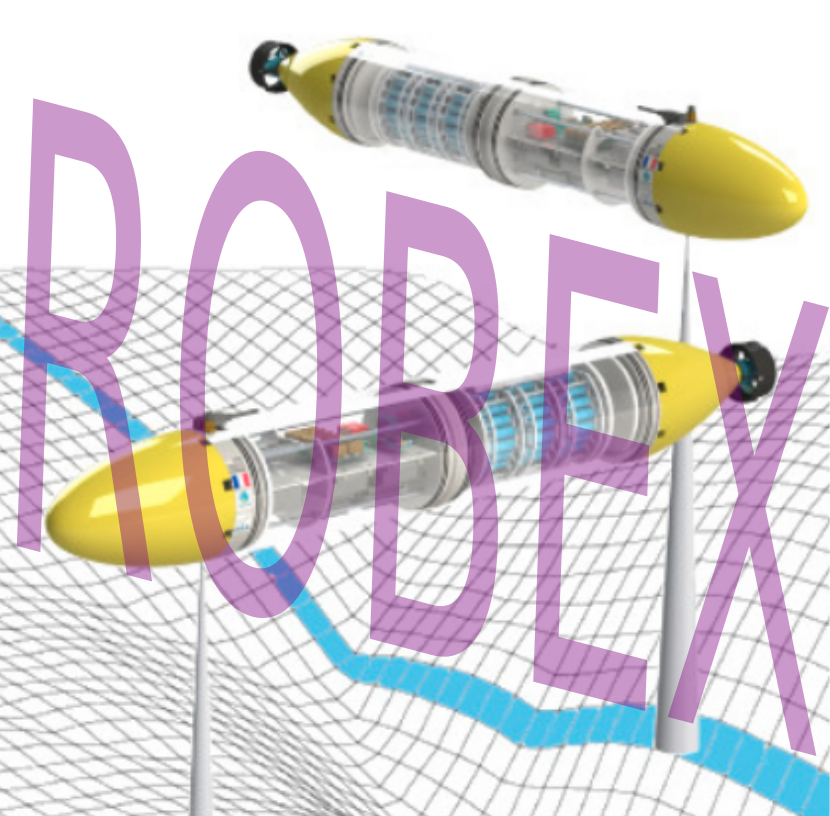
\includegraphics[height=0.6cm]{imgs/logo_robex}}
    \end{tabular}
}

\addtobeamertemplate{frametitle}{}{%
    \begin{tikzpicture}[remember picture,overlay]
    \node[anchor=north east,yshift=2pt] at (current page.north east) {
\includegraphics[height=0.85cm]{imgs/logo_ensta_aid}};
    \end{tikzpicture}
}

\begin{document}

    \maketitle

    \section{Context}

        \begin{frame}{Introduction}{PhD}
            \centering
            \begin{minipage}[c]{0.58\textwidth}
                \begin{block}{Research laboratory}
                    \vspace{0.2cm}
                    \begin{itemize}
                        \item ENSTA Bretagne, UMR 6285, Lab-STICC
                    \end{itemize}
                \end{block}

                \begin{block}{Supervisiors}
                    \begin{itemize}
                        \item Luc Jaulin
                        \item Fabrice Le Bars
                    \end{itemize}
                \end{block}

                \begin{block}{Funding}
                    \begin{itemize}
                        \item AID funding: Jean-Daniel Masson
                    \end{itemize}
                \end{block}
            \end{minipage}
            \hfill
            \begin{minipage}[c]{0.4\textwidth}
                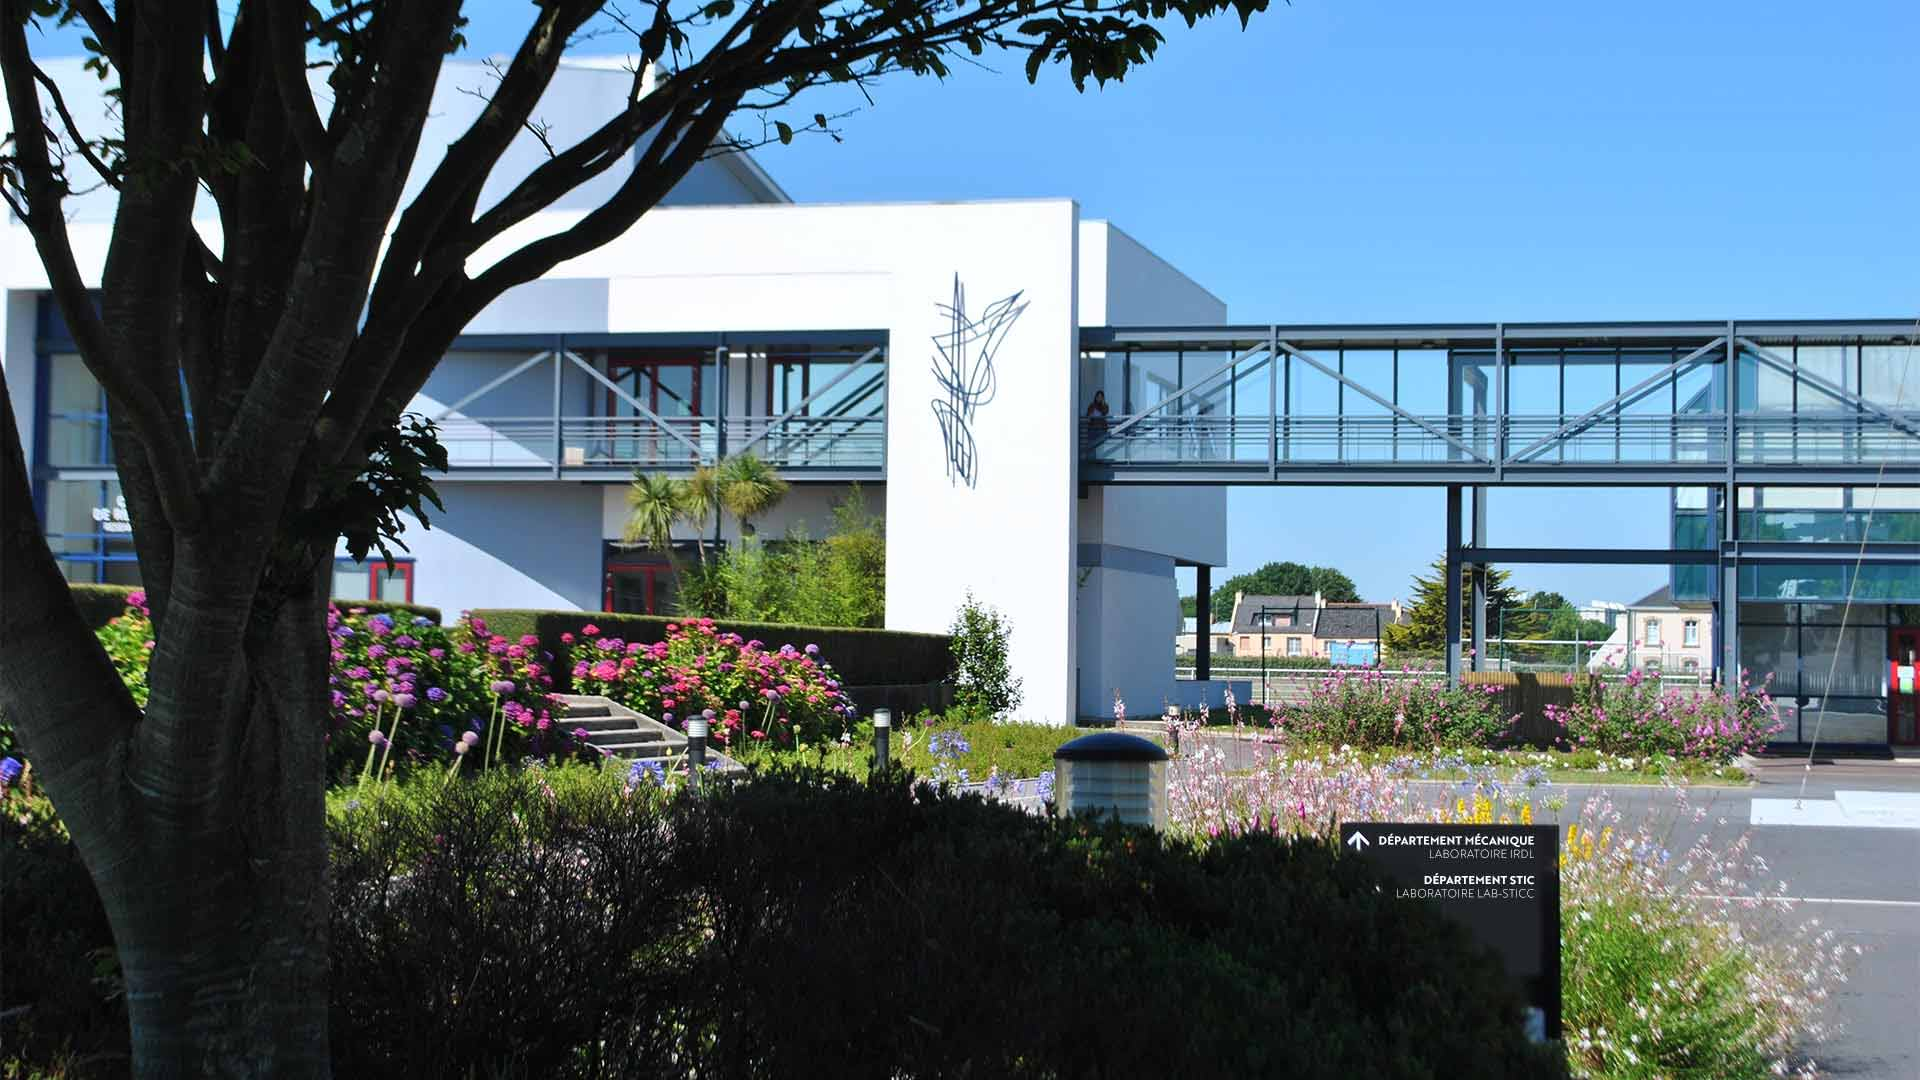
\includegraphics[height=0.7\textheight, trim={24cm 0 16cm 0}, clip]{imgs/ensta.jpg}
            \end{minipage}
        \end{frame}

        \begin{frame}{Introduction}
            \begin{minipage}[c]{0.55\textwidth}
                \begin{block}{AUV}
                    \vspace{0.25cm}
                    \begin{itemize}
                        \item Control of torpedo-like AUV \\ 
                        \item Riptide's micro-uuv
                    \end{itemize}
                \end{block}
                \begin{block}{Environment}
                    \begin{itemize}
                        \item Constrained environment \\ 
                        \item Pool, harbor, ...
                    \end{itemize}
                \end{block}
                \begin{block}{Goals}
                    \begin{itemize}
                        \item Reactivity \\
                        \item Manoeuvrability
                    \end{itemize}
                \end{block}
            \end{minipage}
            \hfill
            \begin{minipage}[c]{0.4\textwidth}
                \begin{figure}[htb]
                    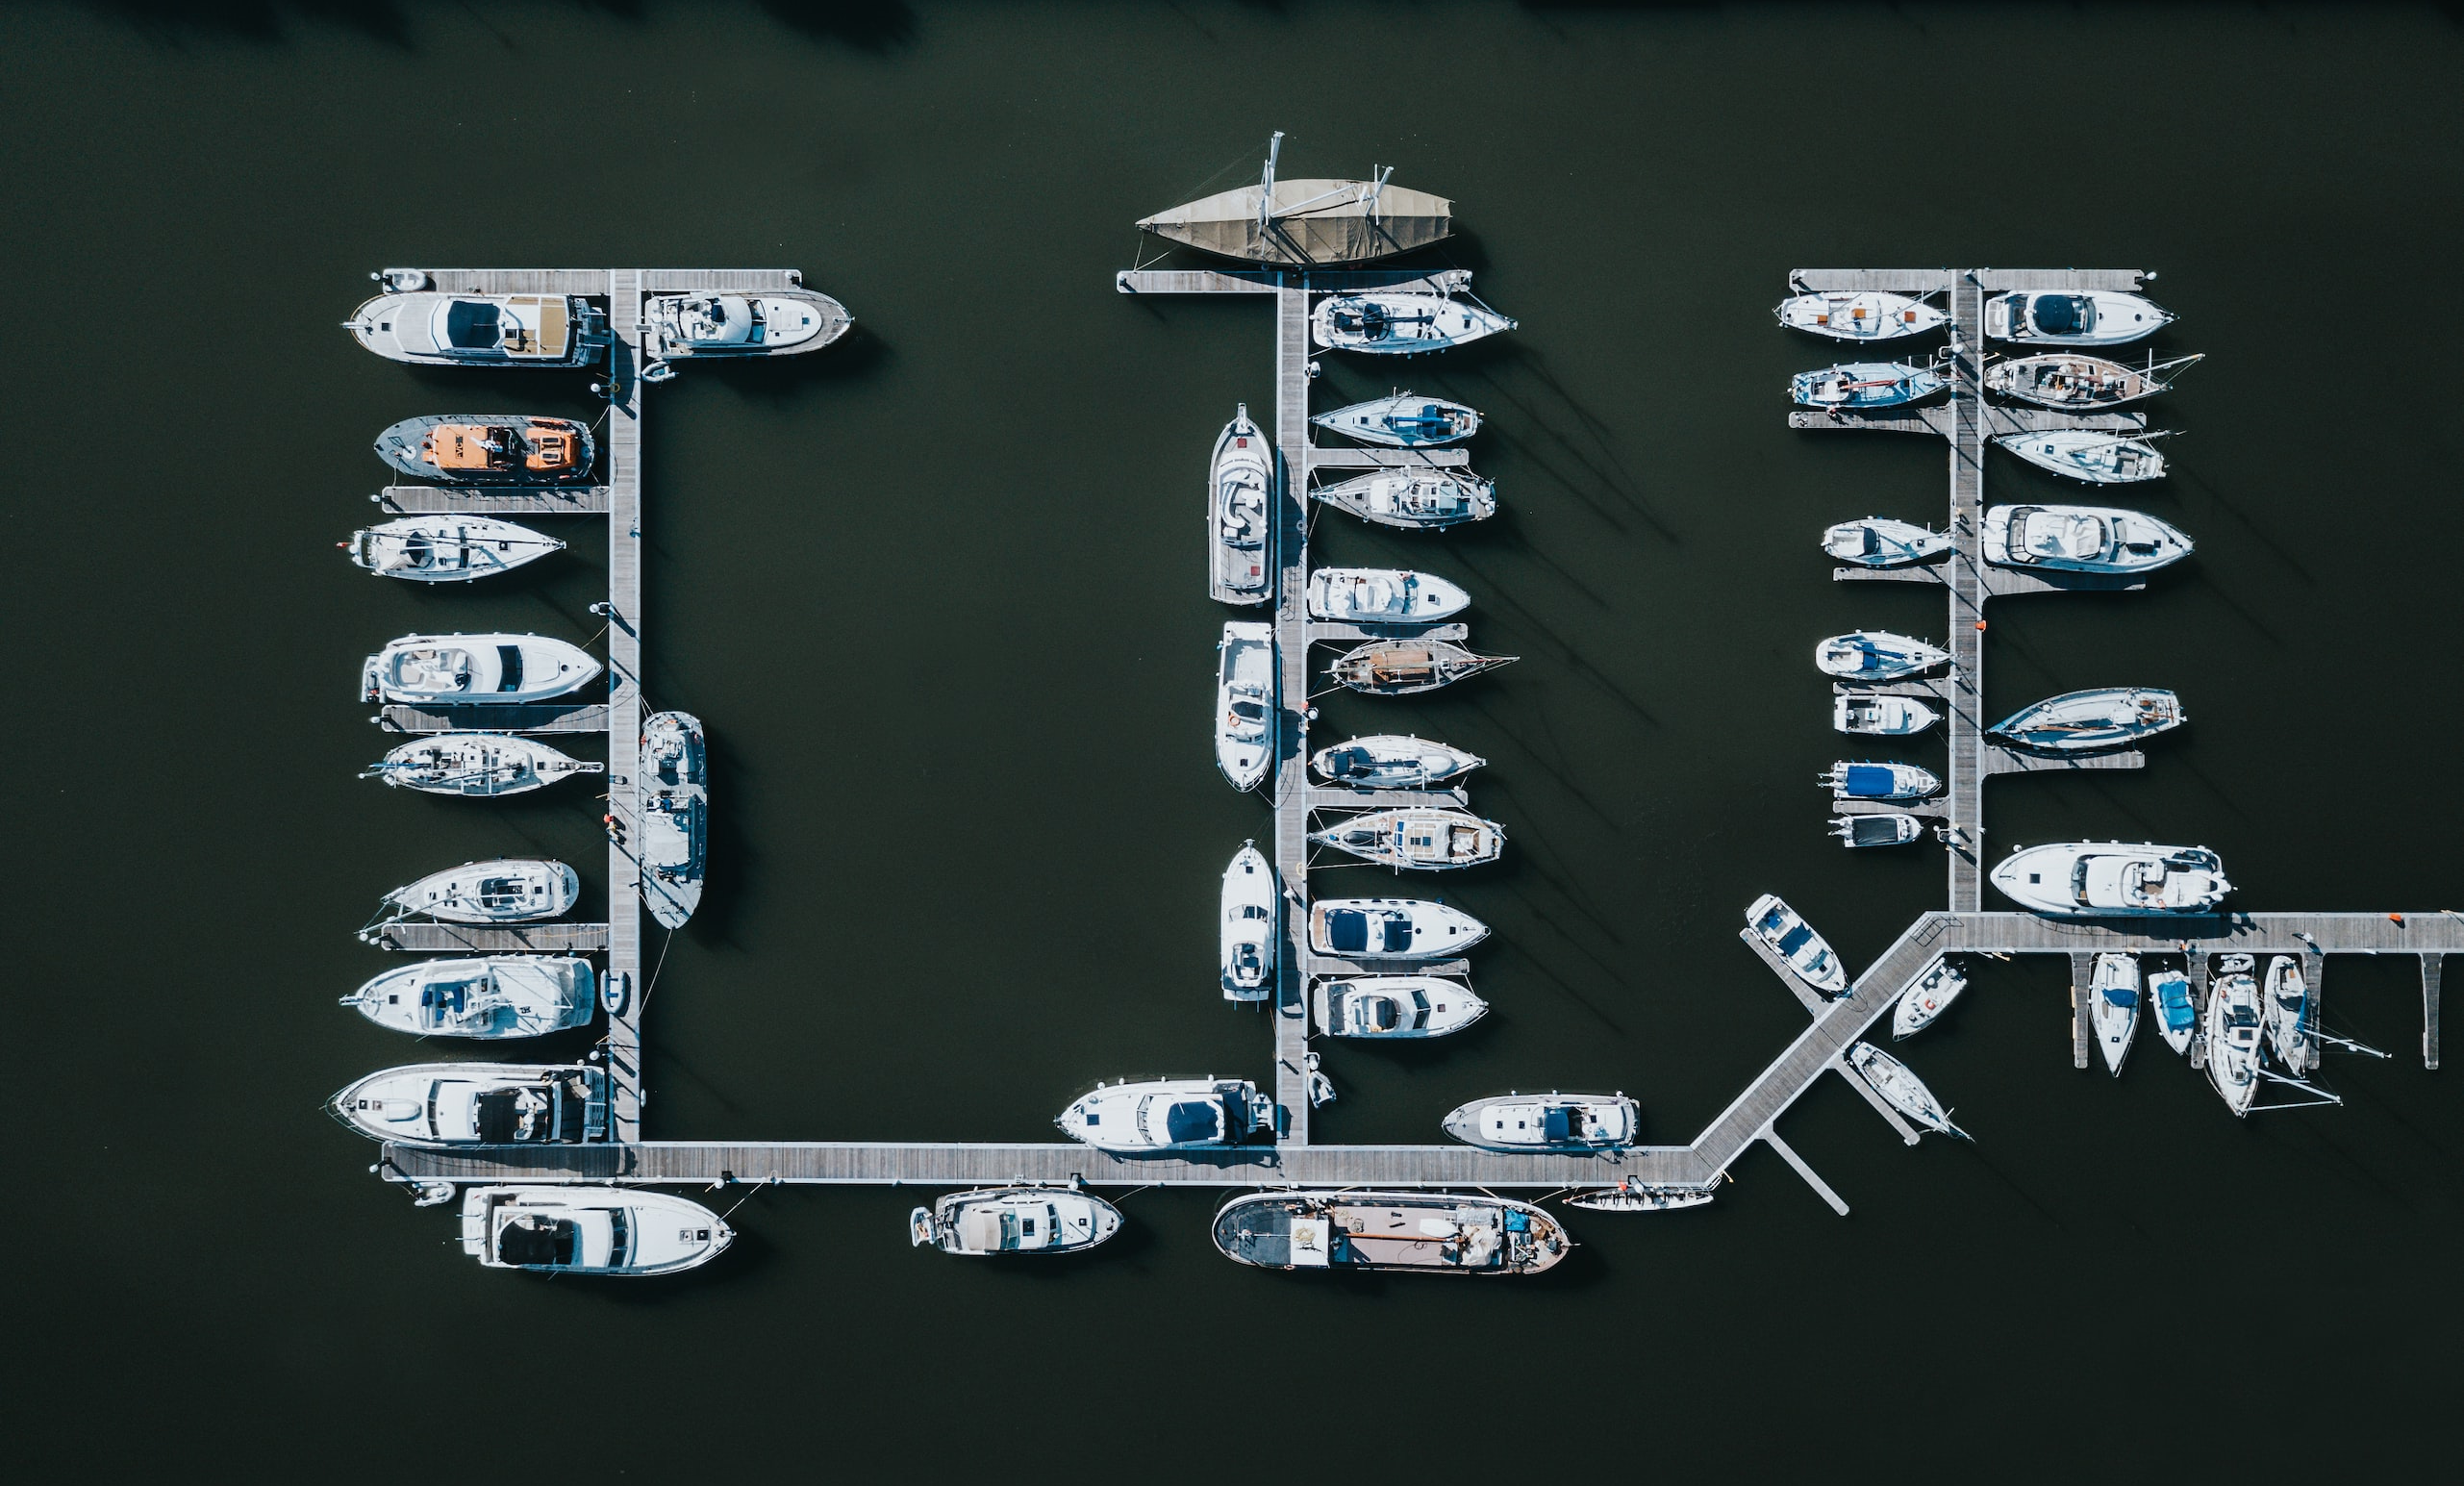
\includegraphics[width=\textwidth]{imgs/harbour.png}

                    \vspace{.1cm}

                    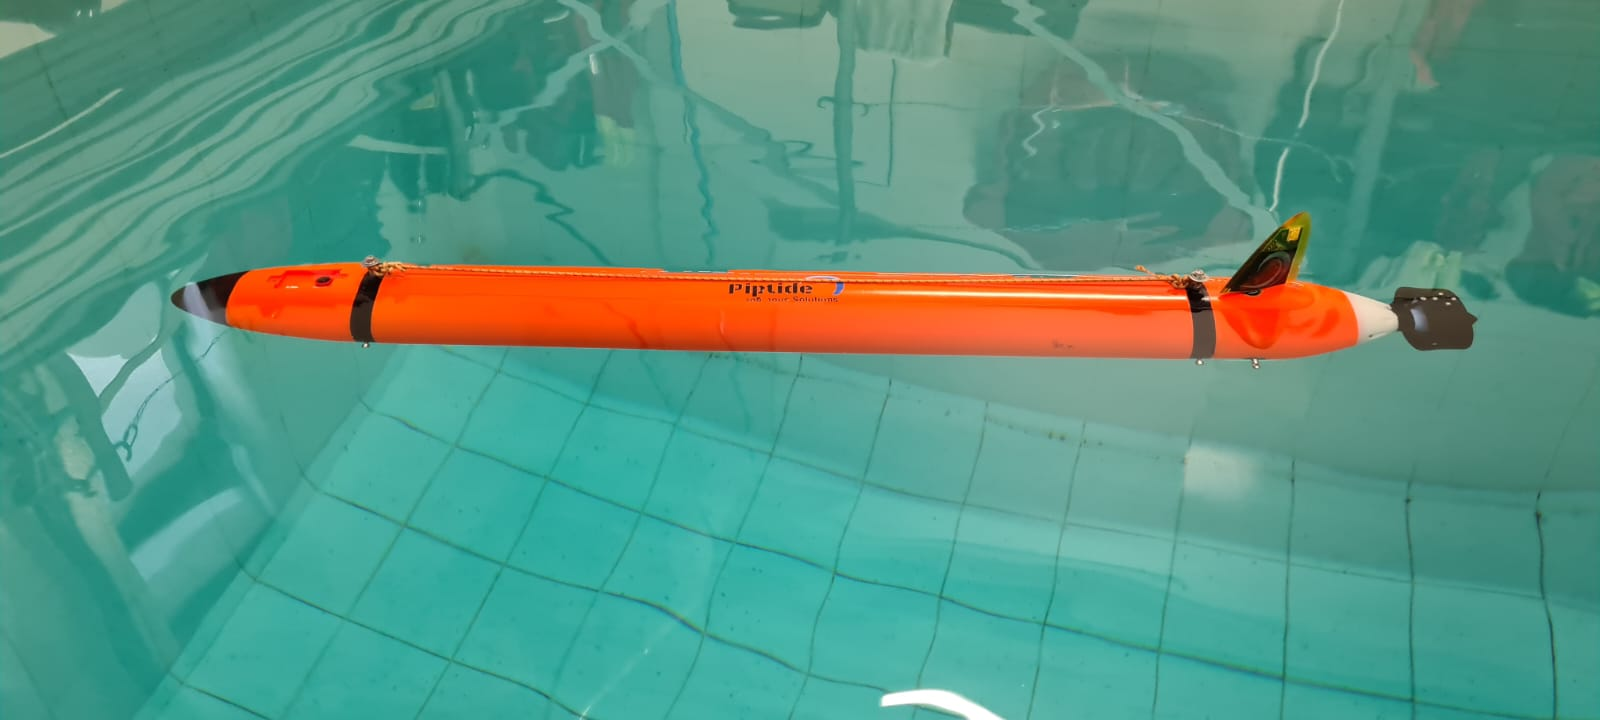
\includegraphics[width=\textwidth]{imgs/Riptide.jpeg}
                    \caption{Harbor and Riptide in the ENSTA Bretagne pool}
                \end{figure}
            \end{minipage}
        \end{frame}

    \section{Motivation}

        \begin{frame}{Orientation control}
            \centering
            \begin{minipage}[c]{0.6\textwidth}
                \begin{block}{Log control}
                    \begin{itemize}
                        \vspace{0.25cm}
                        \item Introduce \textbf{Log control}
                        \item Simple control law \\
                        \item Control AUV orientation \\
                        \item Fastest reorientation
                    \end{itemize}
                \end{block}
            \end{minipage}
        \end{frame}

        \begin{frame}{Log control}
            \centering
            \begin{minipage}{0.45\textwidth}
                \centering
                \begin{figure}
                    \begin{tikzpicture}[
                        wavy/.style={->,>=latex,thick,decorate,
                        decoration={snake,amplitude=2mm,segment length=8mm,pre length=1mm, post length=1mm}}
                        ]
                        \shade[ball color = gray!40, opacity = 0.4] (0,0) circle (2cm);
                        \draw[thick] (0,0) circle (2cm);
                        \onslide<1->{
                            \begin{scope}
                                \draw[thick] (-2,0) arc (180:360:2 and 0.6) coordinate[pos=0.3] (R3);
                                \draw[dashed] (2,0) arc (0:180:2 and 0.6);
                            \end{scope}
                        }
                        \onslide<2->{
                            \coordinate (R1) at (0.8,1.3);
                            \draw[thick,red,->,>=latex] (0,0) -- node[midway,above left] {$\mathbf{u}$} (R1); 
                        }
                        \onslide<3->{
                            \draw[thick,RoyalBlue,->,>=latex] (0,0) -- node[midway,above] {$\mathbf{v}$} (R3);
                        }
                        \coordinate (R4) at (-0.8,1.3);
                        \onslide<4>{
                            \draw[wavy,ForestGreen] (R1) to[bend right=45] (R3);
                            \node[ForestGreen] at (R4) {$\mathbf{w}$};
                        }
                        \onslide<5->{
                            \path[thick,->,>=latex,RoyalPurple] (R1) edge[in=90,out=130] (R3);
                            \node[RoyalPurple] at (R4) {$\mathbf{w}$};
                        }
                    \end{tikzpicture}
                    \caption{Representation in $S^2$}
                \end{figure}
            \end{minipage}
            \hfill
            \begin{minipage}{0.45\textwidth}
                \centering
                \begin{figure}
                    \begin{tikzpicture}[
                        wavy/.style={->,>=latex,thick,decorate,
                        decoration={snake,amplitude=2mm,segment length=8mm,pre length=1mm, post length=1mm}}
                        ]
                        \shade[ball color = gray!40, opacity = 0.4] (0,0) circle (2cm);
                        \draw[thick] (0,0) circle (2cm);
                        \onslide<1->{
                            \begin{scope}
                                \draw[thick] (-2,0) arc (180:360:2 and 0.6) coordinate[pos=0.3] (R3);
                                \draw[dashed] (2,0) arc (0:180:2 and 0.6);
                            \end{scope}
                        }
                        \onslide<3->{
                            \node[thick,RoyalBlue] at (R3) {$\bullet$} node[RoyalBlue] at (R3) [below] {$\mathbf{R_v}$};
                        }
                        \coordinate (R4) at (-0.8,1.3);
                        \onslide<4>{
                            \draw[wavy,ForestGreen,densely dotted] (R1) to[bend right=45] (R3);
                            \node[ForestGreen] at (R4) {$\mathbf{R_w}$};
                        }
                        \onslide<5->{
                            \path[thick,->,>=latex,RoyalPurple,densely dotted] (R1) edge[in=90,out=130] (R3);
                            \node[RoyalPurple] at (R4) {$\mathbf{R_w}$};
                        }
                        \onslide<2->{
                            \coordinate (R1) at (0.8,1.3);
                            \node[red] at (R1) {$\bullet$} node[red] at (R1) [below right] {$\mathbf{R_u}$};
                        }
                    \end{tikzpicture}
                    \caption{Representation in $SO(3)$}
                \end{figure}
            \end{minipage}
        \end{frame}

        \begin{frame}{Log control}
            \centering
            \begin{minipage}{0.45\textwidth}
                \centering
                \begin{figure}
                    \begin{tikzpicture}
                        \shade[ball color = gray!40, opacity = 0.4] (0,0) circle (2cm);
                        \draw[thick] (0,0) circle (2cm);
                        \begin{scope}
                            \draw[thick] (-2,0) arc (180:360:2 and 0.6) coordinate[pos=0.3] (R3);
                            \draw[dashed] (2,0) arc (0:180:2 and 0.6);
                        \end{scope}
                        \coordinate (R1) at (0.8,1.3);
                        \coordinate (R4) at (-0.8,1.3);
                        \node[thick,RoyalBlue] at (R3) {$\bullet$} node[RoyalBlue] at (R3) [below] {$\mathbf{R_v}$};
                        \path[thick,->,>=latex,RoyalPurple,densely dotted] (R1) edge[in=90,out=130] (R3);
                        \node[RoyalPurple] at (R4) {$\mathbf{R_w}$};
                        \node[red] at (R1) {$\bullet$} node[red] at (R1) [below right] {$\mathbf{R_u}$};
                    \end{tikzpicture}
                    \caption{Representation in $SO(3)$}
                \end{figure}
            \end{minipage}
            \hfill
            \begin{minipage}{0.5\textwidth}
                \begin{block}<2->{Rotation matrix}
                    \begin{equation}
                        \mathbf{\color{RoyalPurple}R_w} = \mathbf{\color{red}R_u}^T \cdot \mathbf{\color{ForestGreen}R_v}
                    \end{equation}
                \end{block}
                \begin{block}<3->{Angular velocity w}
                    Link between $\mathbf{\color{RoyalPurple}w}$ and $\mathbf{\color{RoyalPurple}R_w}$.
                    \begin{align}
                        \onslide<4->{\mathbf{\color{RoyalPurple}R_w}^{\color{RubineRed}t} &= Exp~\mathbf{\color{RoyalPurple}w} \\}
                        \onslide<5->{\mathbf{\color{RoyalPurple}w} &= {\color{RubineRed}t} \cdot Log~\mathbf{\color{RoyalPurple}R_w} \\}
                        \notag
                    \end{align}
                    \vskip-1.5em
                \end{block}
            \end{minipage}
        \end{frame}

    \section{Implementation}

        \begin{frame}{Controller block diagram}
            \centering
            \begin{figure}
                \begin{tikzpicture}[
                    input/.style={->,>=latex,thick,decorate,
                    decoration={snake,amplitude=.4mm,segment length=2mm,post length=2mm}},
                    block/.style={draw,font=\small,thick,
                        minimum width={2cm},minimum height={1.5cm}}]

                    \onslide<1-> \node[block,rectangle,align=center] (n3) {AUV\footnote{\textcite{fossen2011handbook}}};

                    \onslide<2->{
                        \node[block,circle,left=of n3] (n2) {Controller};
                        \coordinate (twist) at (n2.west);
                        \foreach \i/\a/\s in {0/37.5/-2.4,1/12.5/-3,2/-12.5/-3,3/-37.5/-2.5} {
                            \draw[thick,->,>=latex,Dandelion] (n2.\a) to node[near end,xshift=\s*1mm,yshift=1.5mm] {$u_\i$} ([yshift=0.6cm -\i * 0.4 cm]n3.west);
                        }
                    }

                    \onslide<3->{
                        \node[block,circle,left=of n2] (n1) {Log \linebreak controller};
                        \draw[thick,->,>=latex,RoyalBlue] (n1) to node[midway,above] {$\mathbf{v}$} node[midway,below] {$\mathbf{w}$} (twist);
                    }

                    % Inputs
                    \onslide<4-6>{
                        \coordinate[above=of n1.100] (u);
                        \draw[input,red] (u) -- node[midway,left,red] {$\mathbf{R_u}$} (n1.100);
                    }
                    \onslide<5-6>{
                        \coordinate[above=of n1.80] (v);
                        \draw[input,ForestGreen] (v) -- node[midway,right,ForestGreen] {$\mathbf{R_v}$} (n1.80);
                    }
                    \onslide<6->{
                        \coordinate(t) at ([shift=({145:2 cm})]n1);
                        \draw[input,RubineRed] (t) -- node[midway,below left,RubineRed] {$\mathbf{t}$} (n1.145);
                    }

                    \onslide<7->{
                        \node[yshift=-0.8cm,red] (Ru) at (n2.south) {$\mathbf{R_u}$};
                        \draw[thick,red,->,>=latex] (n3.south) |- ($(Ru)+(0,0.3)$) -| (n1.south);
                        \coordinate[above=of n1.90] (v);
                        \draw[input,ForestGreen] (v) -- node[midway,right,ForestGreen] {$\mathbf{R_v}$} (n1.90);
                    }
                \end{tikzpicture}
                \caption{
                    \only<1-6>{Open-loop}\only<7->{Closed-loop} block diagram - Log controller
                }
            \end{figure}
        \end{frame}

    \section{Mission}

        \begin{frame}{Mission description}
            \sisetup{input-digits = 0123456789\infty}
            \centering
            \begin{minipage}[c]{0.4\textwidth}
                \centering
                \begin{table}
                    \begin{tabular}[t]{ccc}
                        \toprule
                        State & Depth & Duration \\
                        \midrule
                        $q_0$ & $\qty{0}{\m}$ & $\qty{\infty}{\s}$ \\
                        % \AC{red} \hdashline[.6pt/1.2pt] \EAC
                        $q_1$ & $\qty{3}{\m}$ & $\qty{10}{\s}$ \\
                        $q_2$ & $\qty{1}{\m}$ & $\qty{10}{\s}$ \\
                        $q_3$ & $\qty{3}{\m}$ & $\qty{10}{\s}$ \\
                        \bottomrule
                    \end{tabular}
                    \caption{States description}
                \end{table}
            \end{minipage}
            \hfill
            \begin{minipage}[c]{0.55\textwidth}
                \begin{figure}[\textwidth]
                    \centering
                    \begin{tikzpicture}[node distance=2cm,on grid,auto]
                        \node[state, initial, accepting] (q0) {$q_0$};
                        \node[state, above right of=q0] (q1) {$q_1$};
                        \node[state, below right of=q0] (q3) {$q_3$};
                        \node[state, below right of=q1] (q2) {$q_2$};
                        
                        \draw[->,>=latex]
                            (q0) edge node[midway, above left] {\color{RubineRed}{trigger}} (q1)
                            (q1) edge node[midway, above right] {$d=\qty{10}{\s}$} (q2)
                            (q2) edge node[midway, below right] {$d=\qty{10}{\s}$} (q3)
                            (q3) edge node[midway, below left] {$d=\qty{10}{\s}$} (q0);
                    \end{tikzpicture}
                    \caption{FSM of the mission}
                \end{figure}
            \end{minipage}
        \end{frame}

    \section{Simulation}

        \begin{frame}{Simulation}
            \centering
            \begin{minipage}[c]{0.95\textwidth}
                \begin{figure}
                    \href{run:simulation.mkv?autostart&loop}{\includegraphics[width=\textwidth]{build/imgs/videos/simulation}}
                    \caption{Mission simulation}
                \end{figure}
            \end{minipage}
        \end{frame}

        \begin{frame}{Data}
            \begin{figure}
                \centering
                \begin{tikzpicture}
                    \small
                    \begin{axis}[
                            width=.48\textwidth,
                            height=.4\textheight,
                            grid=major,
                            grid style={dashed,gray!30},
                            xlabel=Time,
                            ylabel=Depth,
                            x unit=\si{\s},
                            y unit=\si{\m},
                            name=depth
                        ]
                        \addplot[solid,thick,RoyalBlue] table [x expr={\fpeval{\thisrow{pressure_stamp} - 1681203552.}}, y=depth, col sep=comma] {data/simulation.csv};
                    \end{axis}

                    \begin{axis}[
                            xshift=.25cm,
                            width=.48\textwidth,
                            height=.4\textheight,
                            grid=major,
                            grid style={dashed,gray!30},
                            xlabel=Time,
                            ylabel=Fin angle,
                            x unit=\si{\s},
                            y unit=\si{\radian},
                            name=fins,
                            at=(depth.right of north east), anchor=left of north west
                        ]
                        \addplot[solid,thick,ForestGreen] table [x expr={\fpeval{\thisrow{time} - 1681203552.}}, y=p_fin, col sep=comma] {data/simulation.csv};
                        \addplot[solid,thick,RubineRed] table [x expr={\fpeval{\thisrow{time} - 1681203552.}}, y=s_fin, col sep=comma] {data/simulation.csv};
                    \end{axis}

                    \begin{axis}[
                            width=.48\textwidth,
                            height=.4\textheight,
                            grid=major,
                            grid style={dashed,gray!30},
                            xlabel=Time,
                            ylabel=Pressure,
                            x unit=\si{\s},
                            y unit=\si{\pascal},
                            name=pressure,
                            at=(depth.below south west), anchor=above north west
                        ]
                        \addplot[solid,thick,RoyalPurple] table [x expr={\fpeval{\thisrow{pressure_stamp} - 1681203552.}}, y=pressure, col sep=comma] {data/simulation.csv};
                    \end{axis}
                \end{tikzpicture}
                \caption{Mission simulation}
            \end{figure}
        \end{frame}

    \section{Conclusion}

        \begin{frame}{Conclusion}
            \centering
            \begin{minipage}{0.8\textwidth}
                \begin{block}{Log control}
                    \vspace*{.25cm}
                    \begin{itemize}
                        \item Simple and elegant control law
                        \item Fastest reorientation along a geodesic in $SO(3)$
                        \item Applicable in orientation control of various robots 
                        \item Need a complete knowledge of $\mathbf{R}$
                    \end{itemize}
                \end{block}
                \begin{block}{Outlook}
                    \begin{itemize}
                        \item Fix Riptide's hardware
                        \item Field experiments on Riptide
                    \end{itemize}
                \end{block}
            \end{minipage}
        \end{frame}

    \appendix

        \begin{frame}[standout]
            Questions?
        \end{frame}

        \begin{frame}[allowframebreaks]{References}

            \settoggle{bbx:url}{false}
            \settoggle{bbx:doi}{false}
            \settoggle{bbx:eprint}{false}
            \settoggle{bbx:isbn}{false}
            \printbibliography[sorting=nyt]

        \end{frame}

        \begin{frame}{Lie algebra vs Lie group}
            \begin{figure}
                \begin{tikzpicture}
                    % Lie algebra
                    \begin{scope}[xshift=-3cm]
                        \draw[black,inner color=gray!10, outer color=gray!40] (-1.5,1.5) rectangle (1.5,-1.5);
                        \coordinate (I) at (-1.1,-1.1);
                        \coordinate (R1) at (0.6,1.1);
                        \node[RoyalPurple] at (R1) {$\bullet$} node[RoyalPurple] at (R1) [yshift=-0.5cm,xshift=-0.6cm] {\footnotesize$\mathbf{w}\wedge\left(\begin{smallmatrix}0&-w_z&w_y\\w_z&0&-w_x\\-w_y&w_x&0\end{smallmatrix}\right)$};
                        \node[RoyalBlue] at (I) {$\bullet$} node[RoyalBlue] at (I) [above,xshift=0.5cm] {\footnotesize$\mathbf{a}\wedge\left(\begin{smallmatrix}0&0&0\\0&0&0\\0&0&0\end{smallmatrix}\right)$};
                        \coordinate (LAr) at (1.5,0);
                        \coordinate (LAb) at (-0.75,-1.5);
                    \end{scope}

                    % Lie group
                    \begin{scope}[scale=0.9,xshift=3cm]
                        \shade[ball color = gray!40, opacity = 0.4] (0,0) circle (2cm);
                        \draw[thick] (-2,0) arc (180:360:2 and 0.6) coordinate[pos=0.3] (I);
                        \draw[dashed] (2,0) arc (0:180:2 and 0.6);
                        \draw[thick] (0,0) circle (2cm);
                        \coordinate (R1) at (-0.6,1.1);
                        \node[RoyalPurple] at (R1) {$\bullet$} node[RoyalPurple] at (R1) [yshift=-0.5cm,xshift=0.6cm] {\footnotesize$\mathbf{R}=exp\left(\begin{smallmatrix}0&-w_z&w_y\\w_z&0&-w_x\\-w_y&w_x&0\end{smallmatrix}\right)$};
                        \node[RoyalBlue] at (I) {$\bullet$} node[RoyalBlue] at (I) [below,xshift=0.5cm] {\footnotesize$\mathbf{I}=exp\left(\begin{smallmatrix}0&0&0\\0&0&0\\0&0&0\end{smallmatrix}\right)$};
                        \coordinate (LGl) at (-2,0);
                        \coordinate (LGb) at (0.75,-2);
                    \end{scope}

                    \begin{scope}[scale=0.18,xshift=-6cm,yshift=-20cm]
                        % The axes
                        \draw[->,>=latex] (xyz cs:x=-2) -- (xyz cs:x=10) node[above] {$x$};
                        \draw[->,>=latex] (xyz cs:y=-2) -- (xyz cs:y=10) node[right] {$z$};
                        \draw[->,>=latex] (xyz cs:z=-10) -- (xyz cs:z=10) node[above] {$y$};

                        % Thin ticks
                        \foreach \coo in {-2,0,...,8} {
                            \draw (\coo,-4pt) -- (\coo,4pt);
                            \draw (-4pt,\coo) -- (4pt,\coo);
                        }
                        \foreach \coo in {-10,-8,...,8} {
                            \draw (xyz cs:y=-0.15pt,z=\coo) -- (xyz cs:y=0.15pt,z=\coo);
                        }
                        
                        % Dashed lines for the points P, Q
                        \draw[dashed] (xyz cs:z=-5) -- +(0,7) coordinate (u) -- (xyz cs:y=7) -- +(5,0) -- 
                            ++(xyz cs:x=5,z=-5) coordinate (v) --+(0,-7) coordinate (w) -- cycle;
                        \draw[dashed] (u) -- (v);
                        \draw[dashed] (5,7) -- (5,0) -- (w);

                        % Dots and labels for P, Q
                        \coordinate (I) at (0,0);
                        \node[RoyalBlue] at (I) {$\bullet$} node[RoyalBlue] at (I) [above,xshift=-0.6cm] {\footnotesize$\mathbf{a}\left(\begin{smallmatrix}0\\0\\0\end{smallmatrix}\right)$};
                        \node[RoyalPurple] at (v) {$\bullet$} node[RoyalPurple] at (v) [right] {\footnotesize$\mathbf{w}\left(\begin{smallmatrix}w_x\\w_y\\w_z\end{smallmatrix}\right)$};

                        \coordinate (Rl) at (-6,2);
                        \coordinate (Rr) at (12,2);
                    \end{scope}

                    \draw[->,>=latex] ([xshift=.25cm,yshift=.25cm]LAr) to [bend left] node [midway,above] {$exp$} ([xshift=-.25cm,yshift=.25cm]LGl);
                    \draw[->,>=latex] ([xshift=-.25cm,yshift=-.25cm]LGl) to [bend left] node [midway,below] {$log$} ([xshift=.25cm,yshift=-.25cm]LAr);
                    
                    \draw[->,>=latex] ([xshift=.25cm,yshift=-.25cm]LAb) to [bend right] node [midway,above right] {$\vee$} ([xshift=-.25cm,yshift=.25cm]Rl);
                    \draw[->,>=latex] ([xshift=-.25cm,yshift=-.25cm]Rl) to [bend left] node [midway,below left] {$\wedge$} ([xshift=-.25cm,yshift=-.25cm]LAb);
                    
                    \draw[->,>=latex] ([xshift=.25cm,yshift=.25cm]Rr) to [bend right] node [midway,above left] {$Exp$} ([xshift=-.25cm,yshift=-.25cm]LGb);
                    \draw[->,>=latex] ([xshift=.25cm,yshift=-.25cm]LGb) to [bend left] node [midway,below right] {$Log$} ([xshift=.25cm,yshift=-.25cm]Rr);

                \end{tikzpicture}
                \caption{Relationship between Lie algebra and Lie group}
            \end{figure}
        \end{frame}

        \begin{frame}{Control}
            \centering
            \begin{minipage}{0.7\textwidth}
                \begin{block}{Control inputs}
                    \centering
                    Controlled physical quantites are linear acceleration $\mathbf{a_r}$ and angular velocity $\mathbf{\omega_r}$
                \end{block}
                \begin{block}{State Equation}
                    \begin{eqnarray}
                        \left\{
                            \begin{array}{rcl}
                                \dot{\mathbf{p}} & = & \mathbf{R} \cdot \mathbf{v_r} \\
                                \dot{\mathbf{R}} & = & \mathbf{R} \cdot (\mathbf{\omega_r} \wedge) \\
                                \dot{\mathbf{v_r}} & = & \mathbf{R}^T \cdot g(\mathbf{p}) + \mathbf{a_r} - \mathbf{\omega_r} \wedge \mathbf{v_r}
                            \end{array}
                        \right.
                    \end{eqnarray}
                \end{block}
            \end{minipage}
        \end{frame}


        \begin{frame}{Torpedo model}
            \centering
            \begin{minipage}{0.7\textwidth}
                \begin{block}{Torpedo assumptions}
                    The following statements are equivalent
                    \begin{itemize}
                        \item No side slip effect \\
                        \item No lateral speed
                        \item Velocity along the $\mathnormal{x}$ axis \\
                    \end{itemize}
                \end{block}
                \begin{block}{Torpedo velocity}
                    \begin{equation}
                        \mathbf{v_r} = (v_r, 0, 0)^T
                    \end{equation}
                \end{block}
            \end{minipage}
        \end{frame}

        \begin{frame}{State Equation}
            \centering
            \begin{minipage}{0.7\textwidth}
                \begin{block}{AUV state}
                    The state of the AUV is denoted by $\mathbf{X} = (\mathbf{p}, \mathbf{v_r}, \mathbf{R})$, where:
                    \begin{itemize}
                        \item $\mathbf{p}$ is the position of the AUV \\
                        \item $\mathbf{v_r}$ is the velocity of the AUV in its frame \\
                        \item $\mathbf{R}$ is the rotation matrix between the world and the AUV \\
                    \end{itemize}
                \end{block}
                \begin{block}{State Equation}
                    \begin{eqnarray}
                        \left\{
                            \begin{array}{rcl}
                                \dot{\mathbf{p}} & = & \mathbf{R} \cdot \mathbf{v_r} \\
                                \dot{\mathbf{R}} & = & \mathbf{R} \cdot (\mathbf{\omega_r} \wedge) \\
                                \dot{\mathbf{v_r}} & = & \mathbf{R}^T \cdot g(\mathbf{p}) + \mathbf{a_r}
                            \end{array}
                        \right.
                    \end{eqnarray}
                \end{block}
            \end{minipage}
        \end{frame}

        \begin{frame}{Inputs}
            \centering
            \begin{minipage}{0.7\textwidth}
                \begin{block}{Inputs}
                    \centering
                    Input vector of the system is $\mathbf{u} = (u_0, u_1, u_2, u_3)^T$, where:
                    \begin{itemize}
                        \item $u_0$: thruster velocity \\
                        \item $u_1, u_2, u_3$: fin angles
                    \end{itemize}
                \end{block}
            \end{minipage}
        \end{frame}

        \begin{frame}{Linear acceleration}
            \centering
            \begin{minipage}{0.7\textwidth}
                \begin{block}{Assumptions}
                    \vspace{0.2cm}
                    \begin{itemize}
                        \item Quadratic thrust with velocity
                        \item Quadratic drag with velocity
                    \end{itemize}
                \end{block}
                \begin{block}{Linear acceleration}
                    \begin{equation}
                        \mathbf{a_r} = \underbrace{p_1 \cdot \left(\begin{smallmatrix}u_0 \\ 0 \\ 0 \end{smallmatrix}\right)^2}_{thrust} - \underbrace{p_2 \cdot \mathbf{v_r} \cdot |\mathbf{v_r}|}_{drag}
                    \end{equation}
                \end{block}
            \end{minipage}
        \end{frame}

        \begin{frame}{Angular velocity}
            \centering
            \begin{minipage}{0.8\textwidth}
                \begin{block}{Assumptions}
                    \vspace{0.2cm}
                    \begin{itemize}
                        \item Fin's drag negligible compared to the AUV drag
                        \item Fin's lift used to control the AUV
                        \item Direct response between the fin's angle and the angular velocity
                    \end{itemize}
                \end{block}
                \begin{block}{Angular velocity}
                    \begin{equation}
                        \mathbf{\omega_r} = v_r^{\color{red}{2}} \cdot 
                            \underbrace{
                                \left(
                                \begin{smallmatrix}
                                    -p_3 & -p_3 & -p_3 \\
                                    0 & p_4 \cdot sin(\frac{2\pi}{3}) & -p_4 \cdot sin(\frac{2\pi}{3}) \\
                                    p_4 & p_4 \cdot cos(\frac{2\pi}{3}) & p_4 \cdot cos(\frac{2\pi}{3})
                                \end{smallmatrix}
                                \right)
                            }_{\mathbf{B}(p_3, p_4)} \cdot \left(\begin{smallmatrix}u_1\\ u_2\\ u_3\end{smallmatrix}\right)
                    \end{equation}
                \end{block}
            \end{minipage}
        \end{frame}

        \begin{frame}{Repartition matrix}
            \centering
            \begin{minipage}{0.8\textwidth}
                \begin{block}{Fin's lift}
                    $\forall i \in \{0, 1, 2\}:$
                    \begin{itemize}
                        \item Force $\mathbf{f_i} = \alpha \cdot u_i \cdot v^2 \cdot (0, 1, 0)^T$
                        \item Orientation $\mathbf{R_i} = \mathbf{R_x}\left(\frac{2i\pi}{3}\right)$
                        \item Center of pressure $\mathbf{q_i} = (\mathit{l_x}, 0, \mathit{l_z})^T$
                        \item Torque $\mathbf{\tau_i} = \mathbf{R_i} \cdot \mathbf{q} \wedge \mathbf{f_i}$
                    \end{itemize}
                \end{block}
                \begin{block}{Angular velocity}
                    \begin{equation}
                        \mathbf{\omega_r} = v_r^2 \cdot 
                            \underbrace{
                                \left(
                                \begin{smallmatrix}
                                    -p_3 & -p_3 & -p_3 \\
                                    0 & p_4 \cdot sin(\frac{2\pi}{3}) & -p_4 \cdot sin(\frac{2\pi}{3}) \\
                                    p_4 & p_4 \cdot cos(\frac{2\pi}{3}) & p_4 \cdot cos(\frac{2\pi}{3})
                                \end{smallmatrix}
                                \right)
                            }_{\mathbf{B}(p_3, p_4)} \cdot \left(\begin{smallmatrix}u_1\\ u_2\\ u_3\end{smallmatrix}\right)
                    \end{equation}
                \end{block}
            \end{minipage}
        \end{frame}
    
\end{document}